\chapter{Avaliação dos resultados do experimento}
	\begin{figure}[H]
		\centering
		\caption{\label{fig:compilacao}Resultado da compilação do projeto inteiro.}
		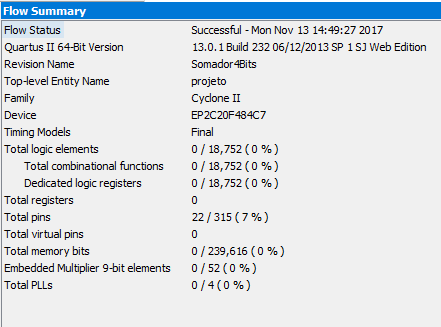
\includegraphics[width=1\textwidth]{img/compilacao}
	\end{figure}

	\section{ETAPA 1 – Display de 7 segmentos}

		Verificou-se, para todos os casos de entrada, que o valor previsto pela \autoref{table:tabelaVerdade1}
		como saída era válido, demonstrando sucesso na implementação do experimento. Isso pode
		ser visualizado tanto pela simulação, como na execução na placa.

		\begin{figure}[H]
		    \centering
			\caption{\label{fig:etapa1Simulacao}Resultado da simulação da etapa 1.}
			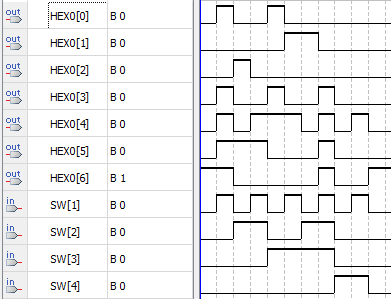
\includegraphics[width=1\textwidth]{img/etapa1/SimulacaoSegmentos7}
		\end{figure}

		\begin{figure}[H]
			\centering

			\begin{subfigure}[b]{0.44\textwidth}
				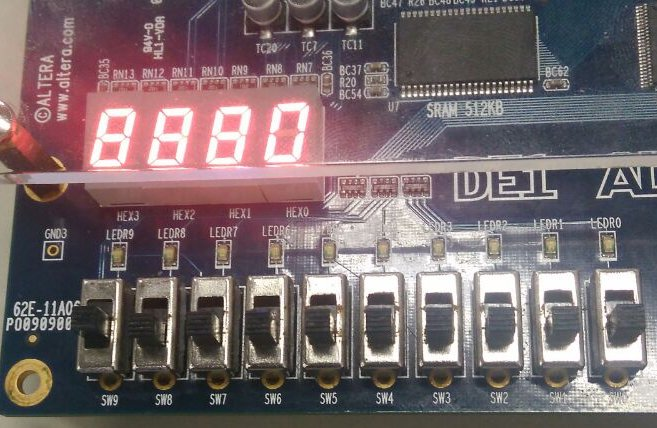
\includegraphics[width=\textwidth]{img/etapa1/0}
				\label{fig:etapa1-0}
				\caption{Número 0}
			\end{subfigure}
			~
			\begin{subfigure}[b]{0.44\textwidth}
				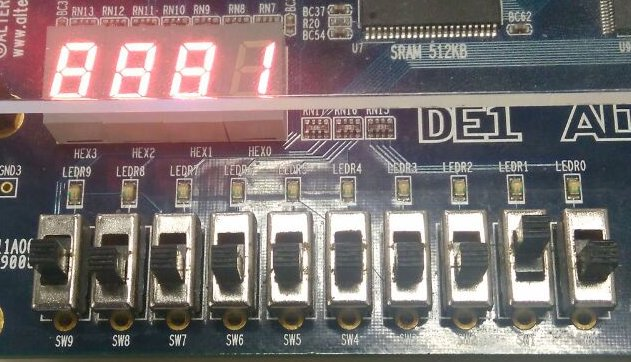
\includegraphics[width=\textwidth]{img/etapa1/1}
				\label{fig:etapa1-1}
				\caption{Número 1}
			\end{subfigure}

			\begin{subfigure}[b]{0.44\textwidth}
				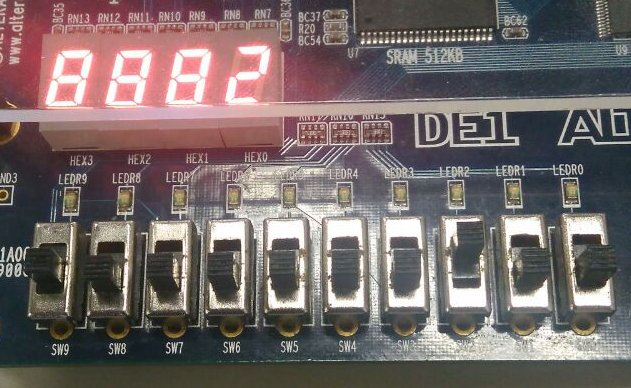
\includegraphics[width=\textwidth]{img/etapa1/2}
				\label{fig:etapa1-2}
				\caption{Número 2}
			\end{subfigure}
			~
			\begin{subfigure}[b]{0.44\textwidth}
				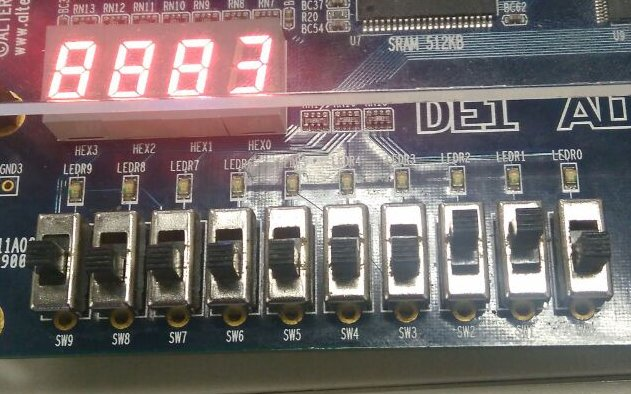
\includegraphics[width=\textwidth]{img/etapa1/3}
				\label{fig:etapa1-3}
				\caption{Número 3}
			\end{subfigure}
			\begin{subfigure}[b]{0.44\textwidth}
				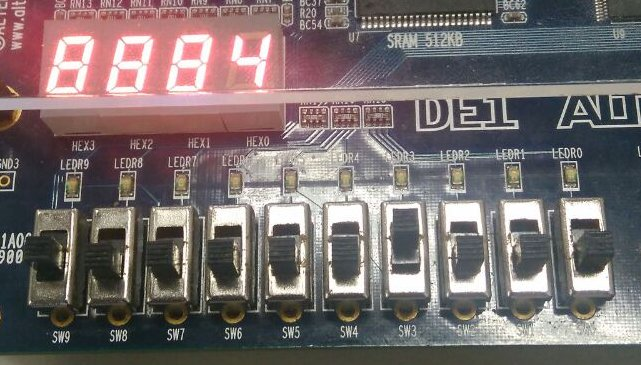
\includegraphics[width=\textwidth]{img/etapa1/4}
				\label{fig:etapa1-4}
				\caption{Número 4}
			\end{subfigure}
			~
			\begin{subfigure}[b]{0.44\textwidth}
				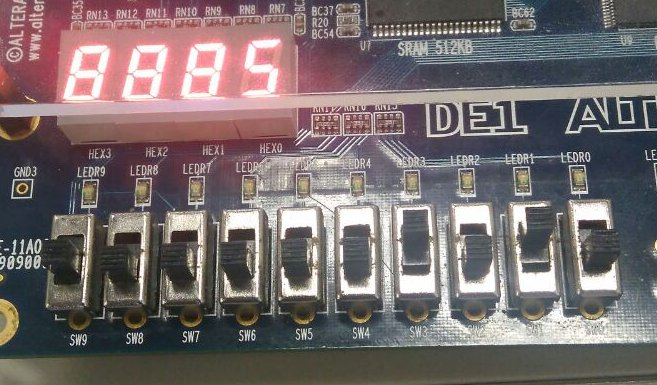
\includegraphics[width=\textwidth]{img/etapa1/5}
				\label{fig:etapa1-5}
				\caption{Número 5}
			\end{subfigure}

			\caption{Teste do circuito rodando na placa, no intervalo de 0-5.}\label{fig:etapa1Teste1}
		\end{figure}

		\begin{figure}[H]
			\centering

			\begin{subfigure}[b]{0.44\textwidth}
				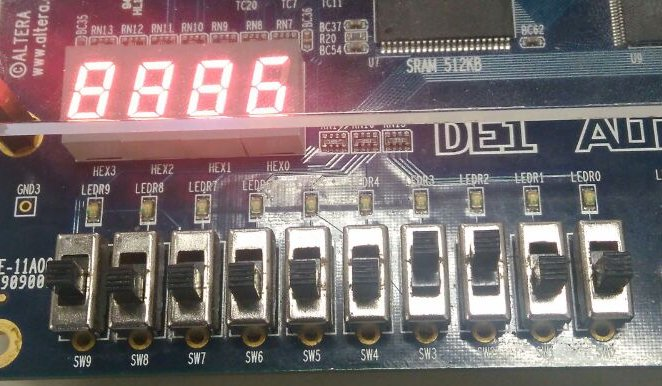
\includegraphics[width=\textwidth]{img/etapa1/6}
				\label{fig:etapa1-6}
				\caption{Número 6}
			\end{subfigure}
			~
			\begin{subfigure}[b]{0.44\textwidth}
				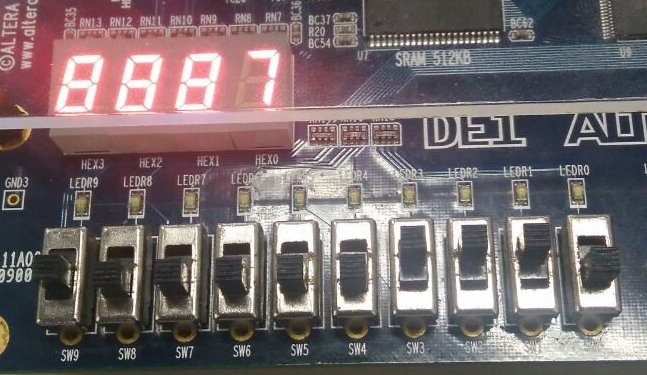
\includegraphics[width=\textwidth]{img/etapa1/7}
				\label{fig:etapa1-7}
				\caption{Número 7}
			\end{subfigure}

			\begin{subfigure}[b]{0.44\textwidth}
				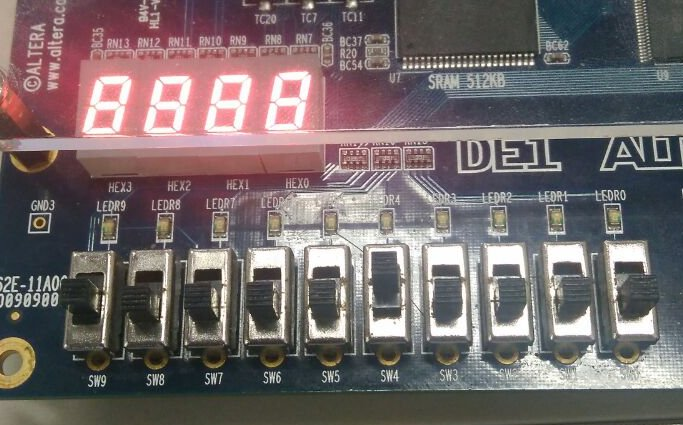
\includegraphics[width=\textwidth]{img/etapa1/8}
				\label{fig:etapa1-8}
				\caption{Número 8}
			\end{subfigure}
			~
			\begin{subfigure}[b]{0.44\textwidth}
				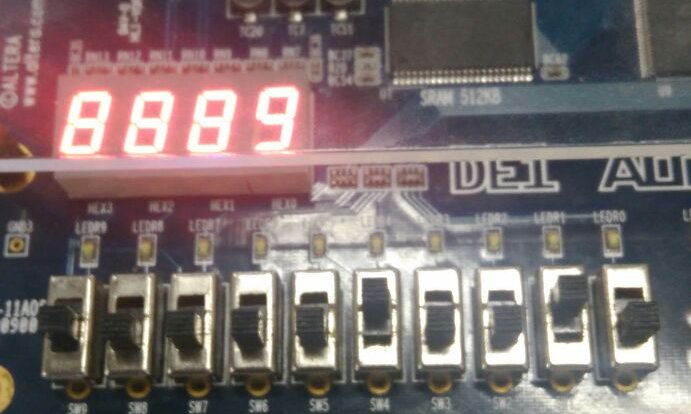
\includegraphics[width=\textwidth]{img/etapa1/9}
				\label{fig:etapa1-9}
				\caption{Número 9}
			\end{subfigure}

			\caption{Teste do circuito rodando na placa, no intervalo de 6-9.}\label{fig:etapa1Teste2}
		\end{figure}


	\section{ETAPA 2 – Meio-somador 1 bit}
		Na etapa 2, o experimento demonstrou os resultados esperados, de acordo com a
		 \autoref{table:tabelaMeioSomador}.

		\begin{figure}[H]
		    \centering
			\caption{\label{fig:etapa2Simulacao}Resultado da simulação da etapa 2.}
			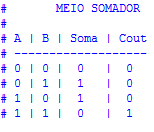
\includegraphics[width=1\textwidth]{img/etapa2/simulacaoMeioSomador}
		\end{figure}

		Após o \textit{deploy} na placa no kit DE1, o kit educacional da Altera, o circuito apresentou
		 os resultados esperados, representando o resultado da soma no display de 7 segmentos HEX0,
		 conforme \autoref{fig:etapa2Teste}.

		\begin{figure}[H]
			\centering

			\begin{subfigure}[b]{0.44\textwidth}
				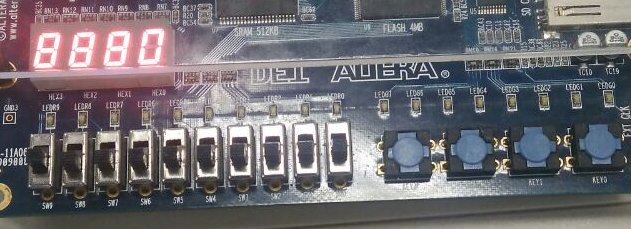
\includegraphics[width=\textwidth]{img/etapa2/00}
				\label{fig:etapa2-00}
				\caption{Entrada 0 0}
			\end{subfigure}
			~
			\begin{subfigure}[b]{0.44\textwidth}
				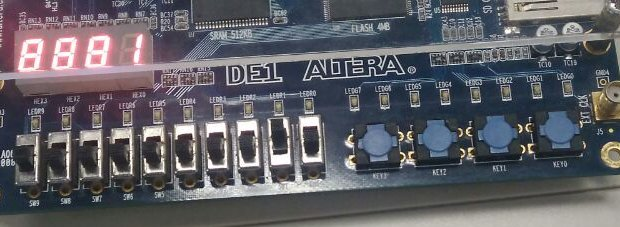
\includegraphics[width=\textwidth]{img/etapa2/01}
				\label{fig:etapa2-01}
				\caption{Entrada 0 1}
			\end{subfigure}

			\begin{subfigure}[b]{0.44\textwidth}
				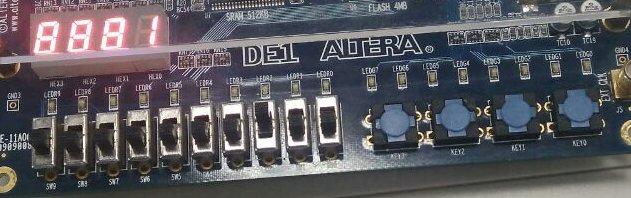
\includegraphics[width=\textwidth]{img/etapa2/10}
				\label{fig:etapa2-10}
				\caption{Entrada 1 0}
			\end{subfigure}
			~
			\begin{subfigure}[b]{0.44\textwidth}
				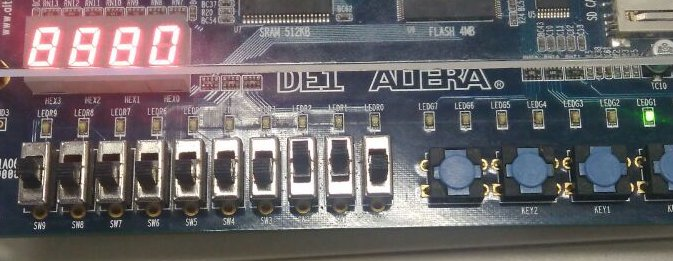
\includegraphics[width=\textwidth]{img/etapa2/11}
				\label{fig:etapa2-11}
				\caption{Entrada 1 1}
			\end{subfigure}

			\caption{Teste do circuito rodando na placa.}\label{fig:etapa2Teste}
		\end{figure}

	\section{ETAPA 3 – Meio-somador 4 bits}

	O resultado foi como o esperado, conforme pode ser visto na simulação, execução na placa e no testbench.
	\begin{figure}[H]
		\centering
		\caption{\label{fig:waveSomadorCompleto}Simulação do projeto.}
		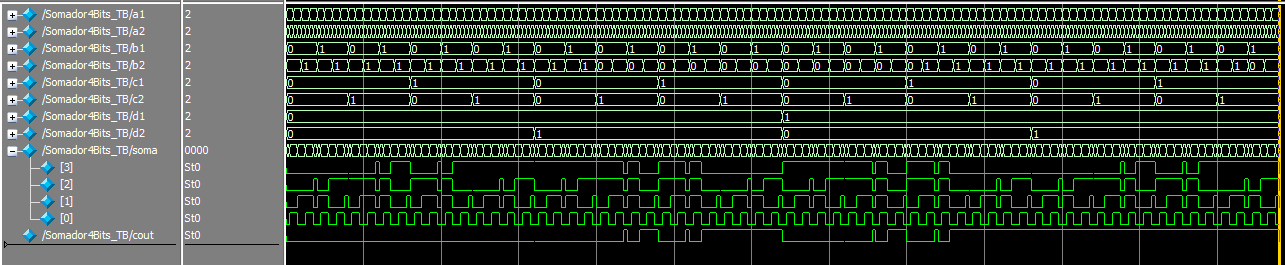
\includegraphics[width=1\textwidth]{img/etapa3/waveSomadorCompleto4Bits}
	\end{figure}

	\begin{figure}[H]
		\centering

		\begin{subfigure}[b]{0.44\textwidth}
			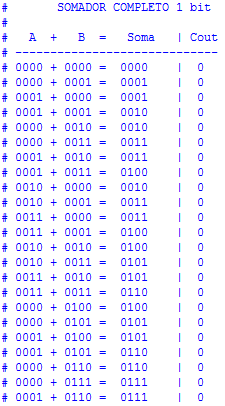
\includegraphics[width=\textwidth]{img/etapa3/simulacaoSomadorCompleto4Bits_1}
			\label{fig:etapa3-1}
		\end{subfigure}
		~
		\begin{subfigure}[b]{0.44\textwidth}
			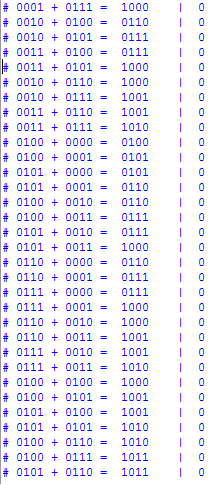
\includegraphics[width=\textwidth]{img/etapa3/simulacaoSomadorCompleto4Bits_2}
			\label{fig:etapa3-2}
		\end{subfigure}

		\begin{subfigure}[b]{0.44\textwidth}
			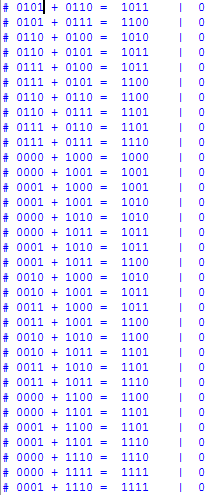
\includegraphics[width=\textwidth]{img/etapa3/simulacaoSomadorCompleto4Bits_3}
			\label{fig:etapa3-3}
		\end{subfigure}
		~
		\begin{subfigure}[b]{0.44\textwidth}
			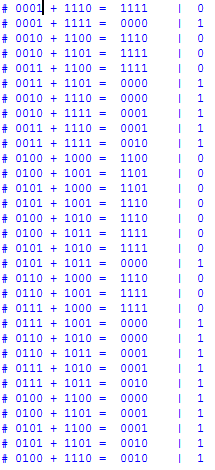
\includegraphics[width=\textwidth]{img/etapa3/simulacaoSomadorCompleto4Bits_4}
			\label{fig:etapa3-4}

		\end{subfigure}

		\begin{subfigure}[b]{0.44\textwidth}
			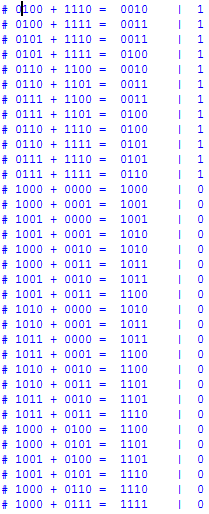
\includegraphics[width=\textwidth]{img/etapa3/simulacaoSomadorCompleto4Bits_5}
			\label{fig:etapa3-5}
		\end{subfigure}
		~
		\begin{subfigure}[b]{0.44\textwidth}
			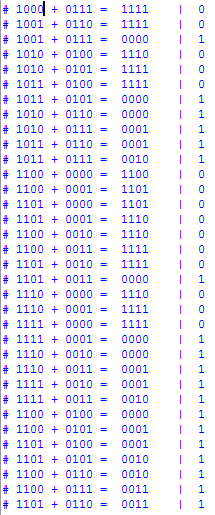
\includegraphics[width=\textwidth]{img/etapa3/simulacaoSomadorCompleto4Bits_6}
			\label{fig:etapa3-6}
		\end{subfigure}

		\begin{subfigure}[b]{0.44\textwidth}
			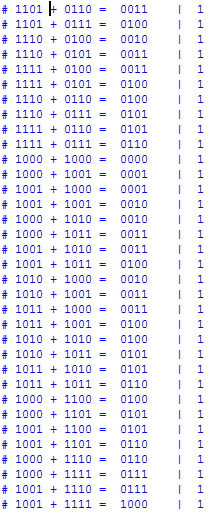
\includegraphics[width=\textwidth]{img/etapa3/simulacaoSomadorCompleto4Bits_7}
			\label{fig:etapa3-7}
		\end{subfigure}
		~
		\begin{subfigure}[b]{0.44\textwidth}
			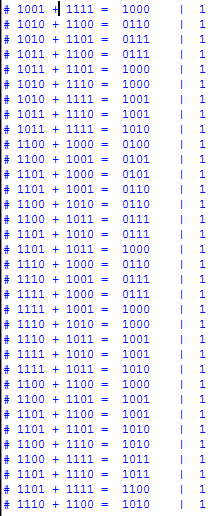
\includegraphics[width=\textwidth]{img/etapa3/simulacaoSomadorCompleto4Bits_8}
			\label{fig:etapa3-8}
		\end{subfigure}

		\begin{subfigure}[b]{0.44\textwidth}
			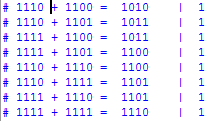
\includegraphics[width=\textwidth]{img/etapa3/simulacaoSomadorCompleto4Bits_9}
			\label{fig:etapa3-9}
		\end{subfigure}

		\caption{Resultado do testbench do projeto completo.}
	\end{figure}

	\begin{figure}[H]
		\centering

		\begin{subfigure}[b]{0.44\textwidth}
			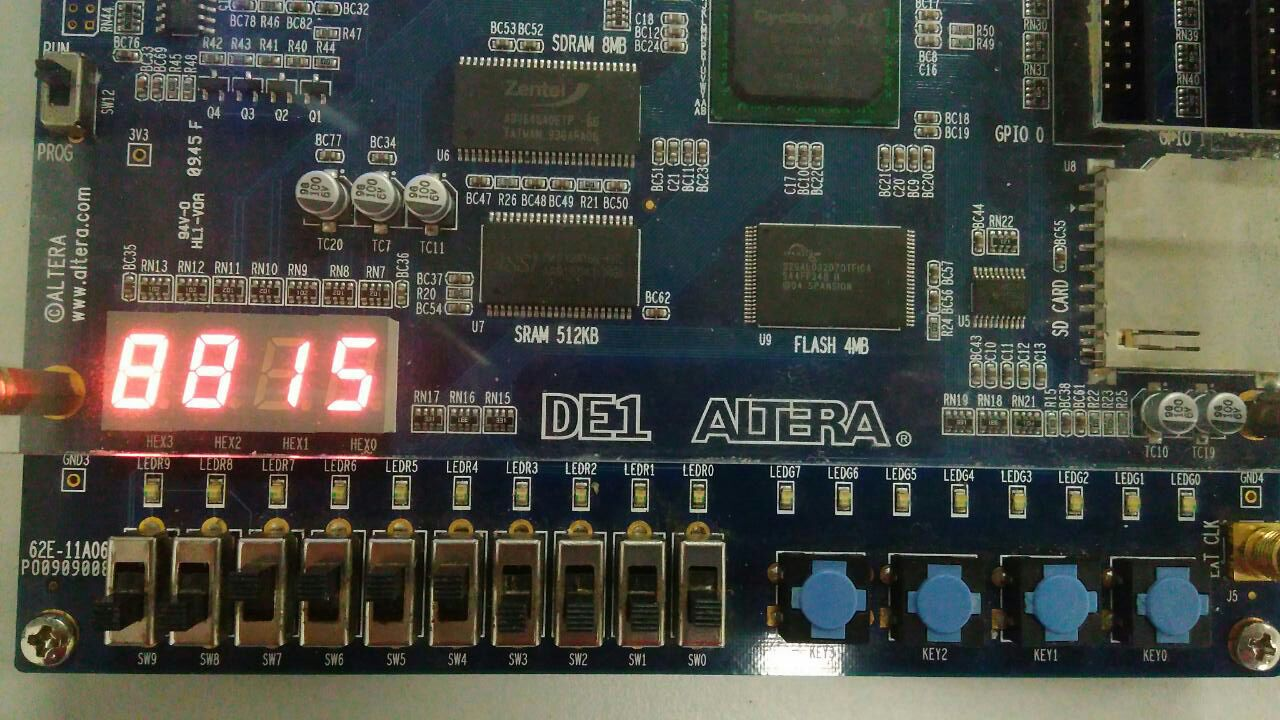
\includegraphics[width=\textwidth]{img/etapa3/1}
			\label{fig:etapa3-10}
		\end{subfigure}
		~
		\begin{subfigure}[b]{0.44\textwidth}
			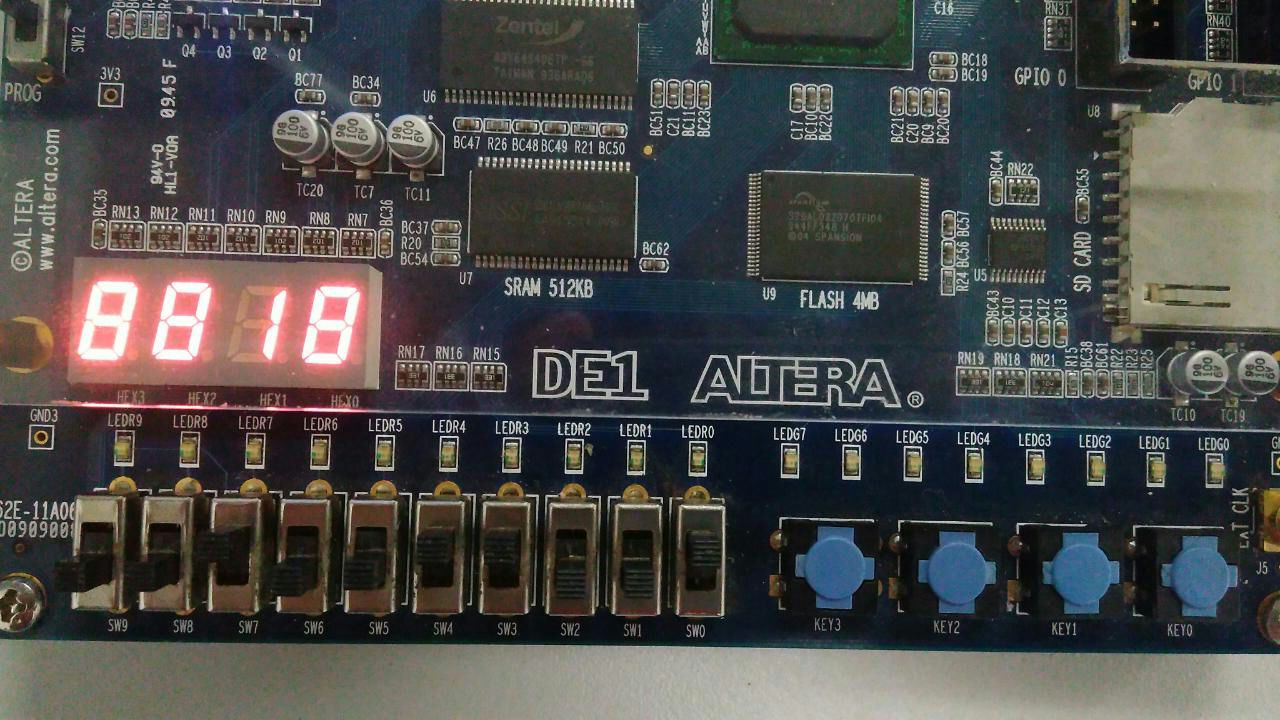
\includegraphics[width=\textwidth]{img/etapa3/2}
			\label{fig:etapa3-11}
		\end{subfigure}

		\begin{subfigure}[b]{0.44\textwidth}
			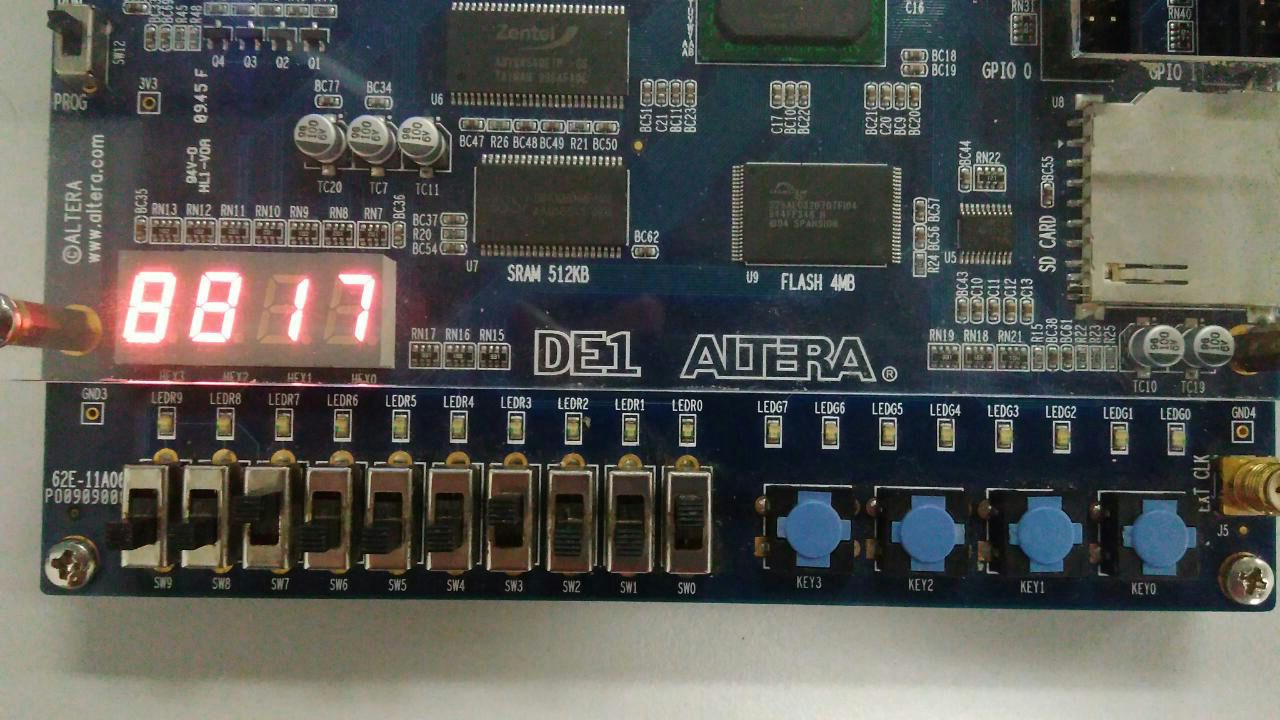
\includegraphics[width=\textwidth]{img/etapa3/3}
			\label{fig:etapa3-12}
		\end{subfigure}
		~
		\begin{subfigure}[b]{0.44\textwidth}
			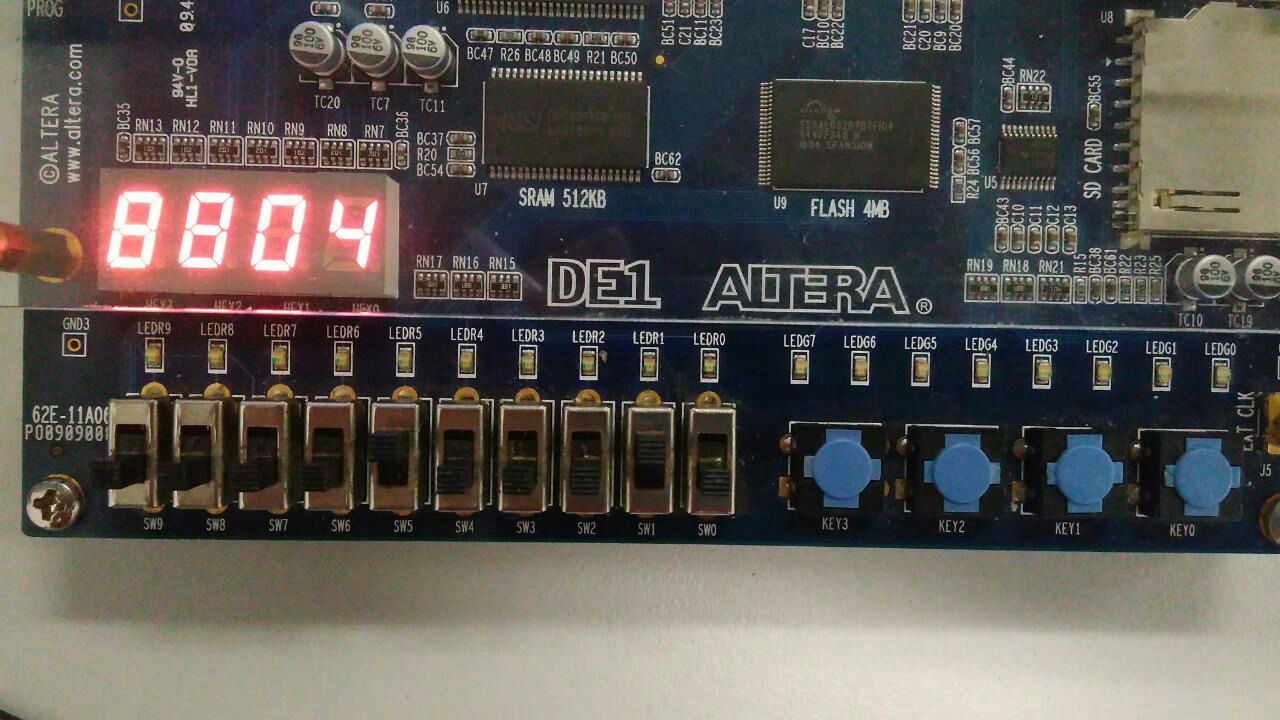
\includegraphics[width=\textwidth]{img/etapa3/4}
			\label{fig:etapa3-13}

		\end{subfigure}

		\begin{subfigure}[b]{0.44\textwidth}
			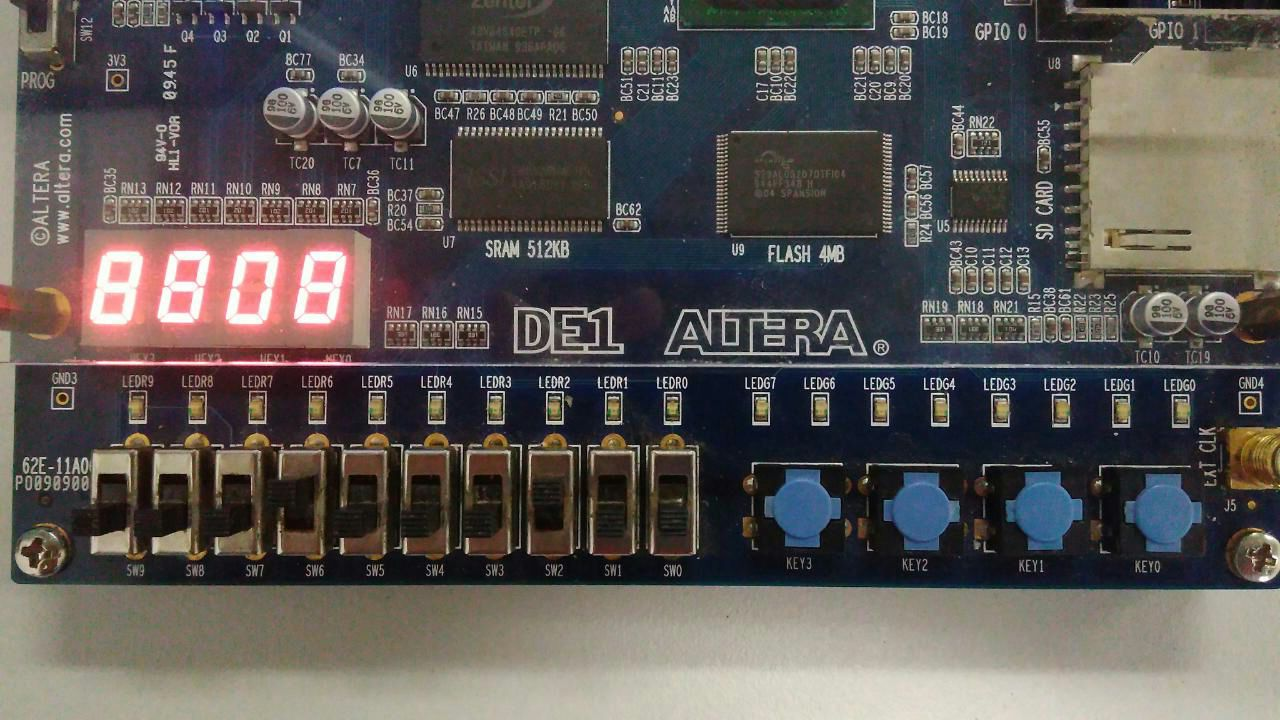
\includegraphics[width=\textwidth]{img/etapa3/5}
			\label{fig:etapa3-14}
		\end{subfigure}
		~
		\begin{subfigure}[b]{0.44\textwidth}
			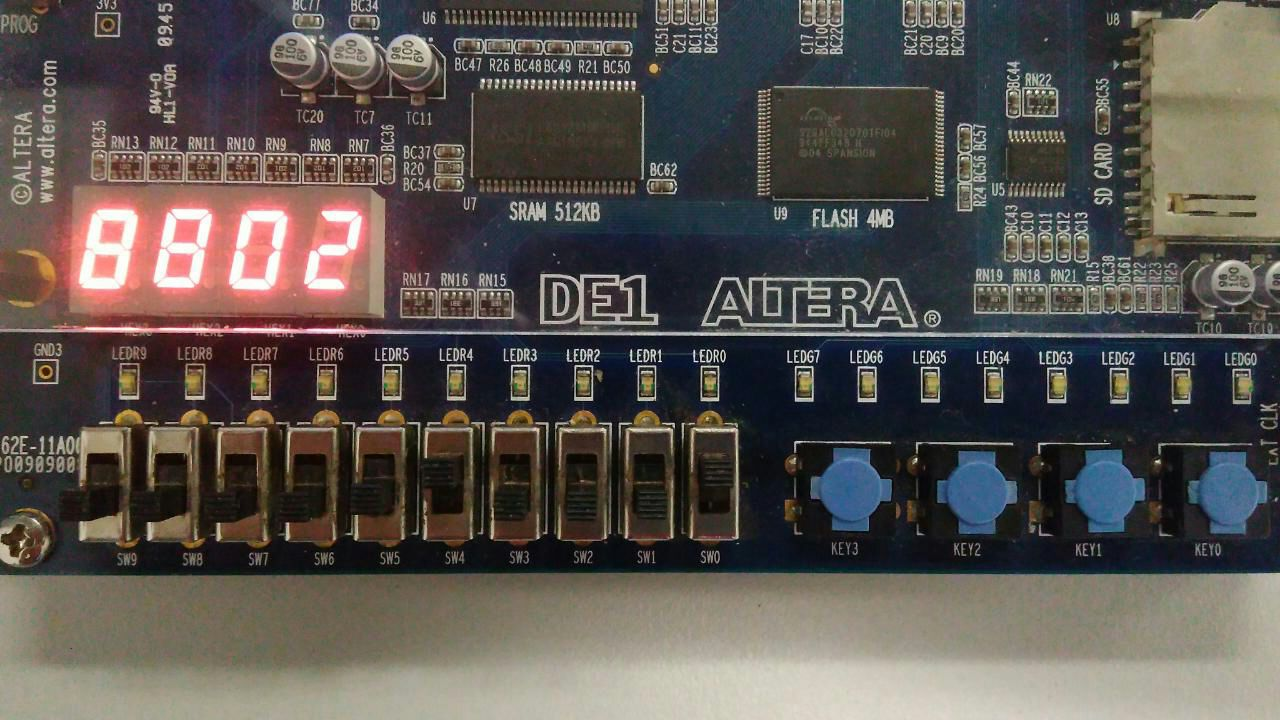
\includegraphics[width=\textwidth]{img/etapa3/6}
			\label{fig:etapa3-15}
		\end{subfigure}

		\begin{subfigure}[b]{0.44\textwidth}
			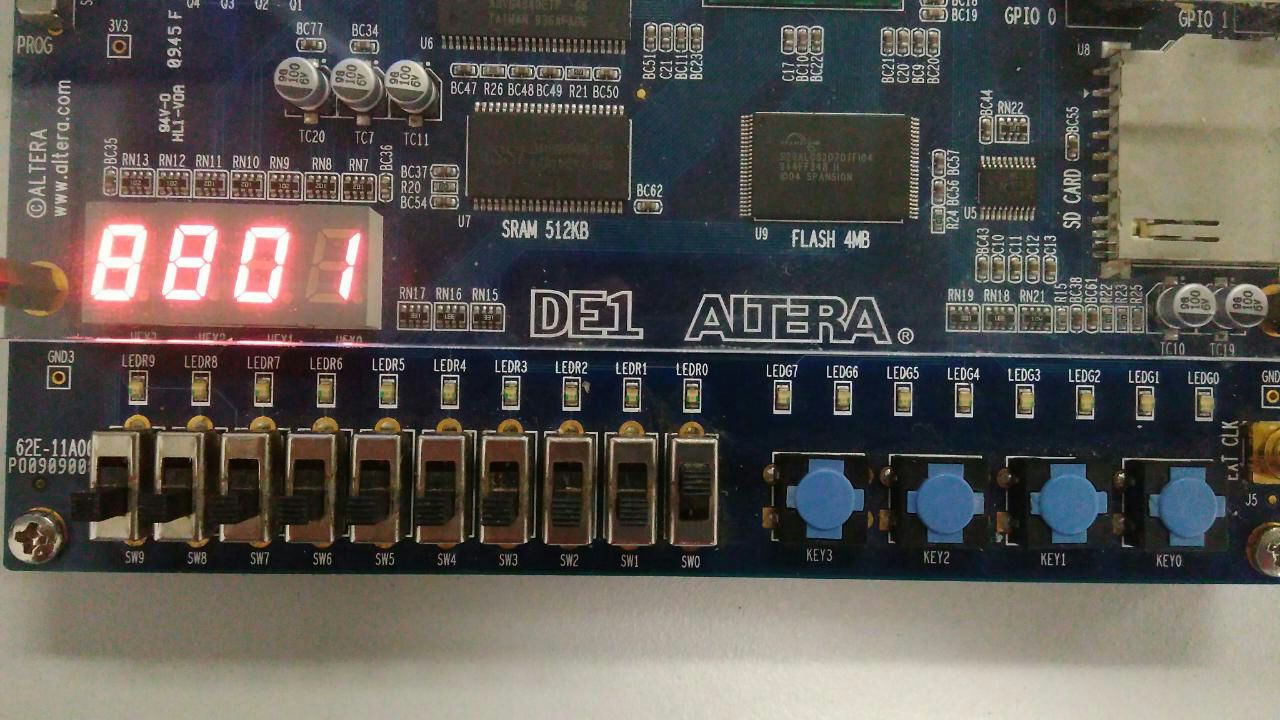
\includegraphics[width=\textwidth]{img/etapa3/7}
			\label{fig:etapa3-16}
		\end{subfigure}
		~
		\begin{subfigure}[b]{0.44\textwidth}
			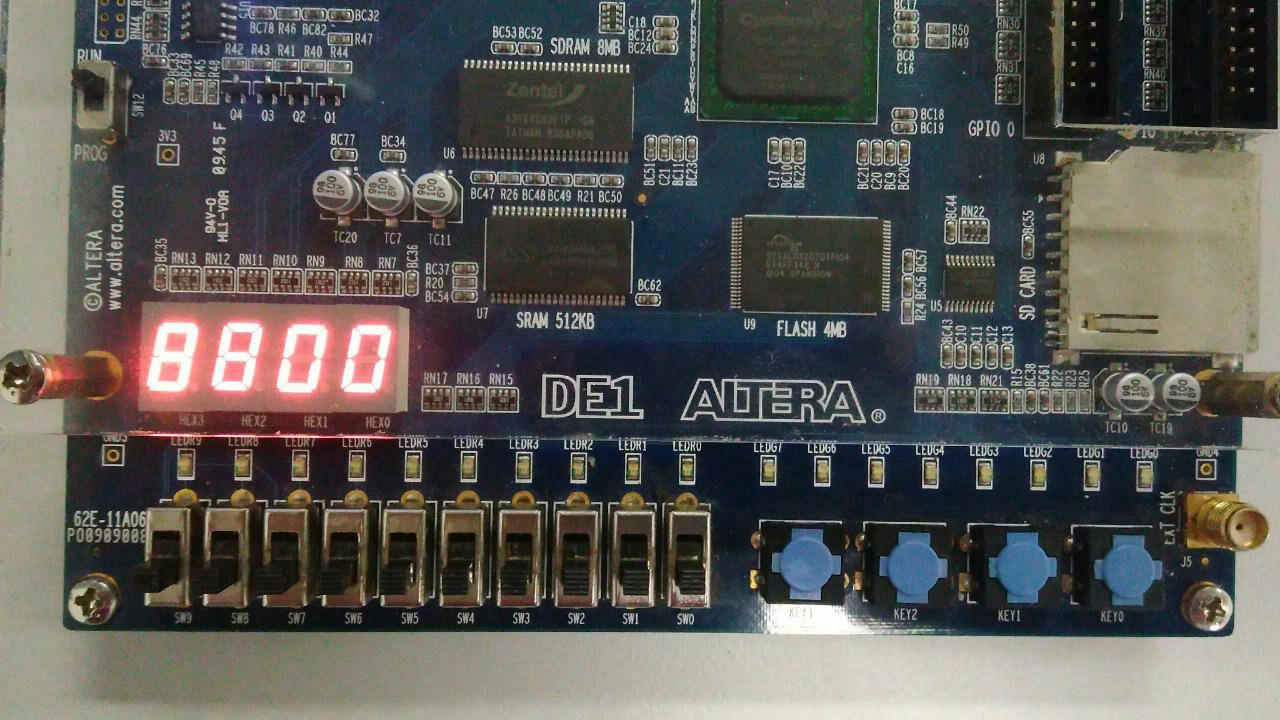
\includegraphics[width=\textwidth]{img/etapa3/8}
			\label{fig:etapa3-17}
		\end{subfigure}

		\caption{Execução do projeto na FPGA.}
	\end{figure}



	Os testbench podem ser encontrados nos apêndices.

%Apresentar os resultados da simulação em software e da utilização do Kit DE1 e/ou
%protoboard. Utilizar figuras, descrevê-las e discuti-las.
